% !TeX root = ../main.tex

\chapter{绪论}

\section{研究背景和意义}

\subsection{研究背景}
随着目前我国整体经济实力和科研水平的快速上升,计算机视觉技术及其大量成熟的现实应用如图像生成,图像去噪,图像分类等已经凭借着充足的资本支撑,庞大的原料准备和精干的队伍建设在科学和经济领域炙手可热,并对依赖其的下游任务如具身智能,自动驾驶创造了巨大的提升空间和美好前景。
而且随着普通场景下视觉任务的逐渐完善,超越常规硬件的高速运动场景带来的运动模糊,变形,失焦等问题逐渐得到关注。特定领域如航天、军事、体育对高速目标的精准识别提出严格要求。传统的高速相机的工作原理是曝光-读取模式,在一定的时间窗口中通过打开快门使得光感受器接受光子,随后关闭快门进行数据读取。
这个时间窗口就被称之为曝光时间。但这种方式本质上牺牲了连续两张图片之间数据读取时的物体运动,因而会带来不可避免地运动信息丢失。

\begin{figure}[ht]
  \centering
  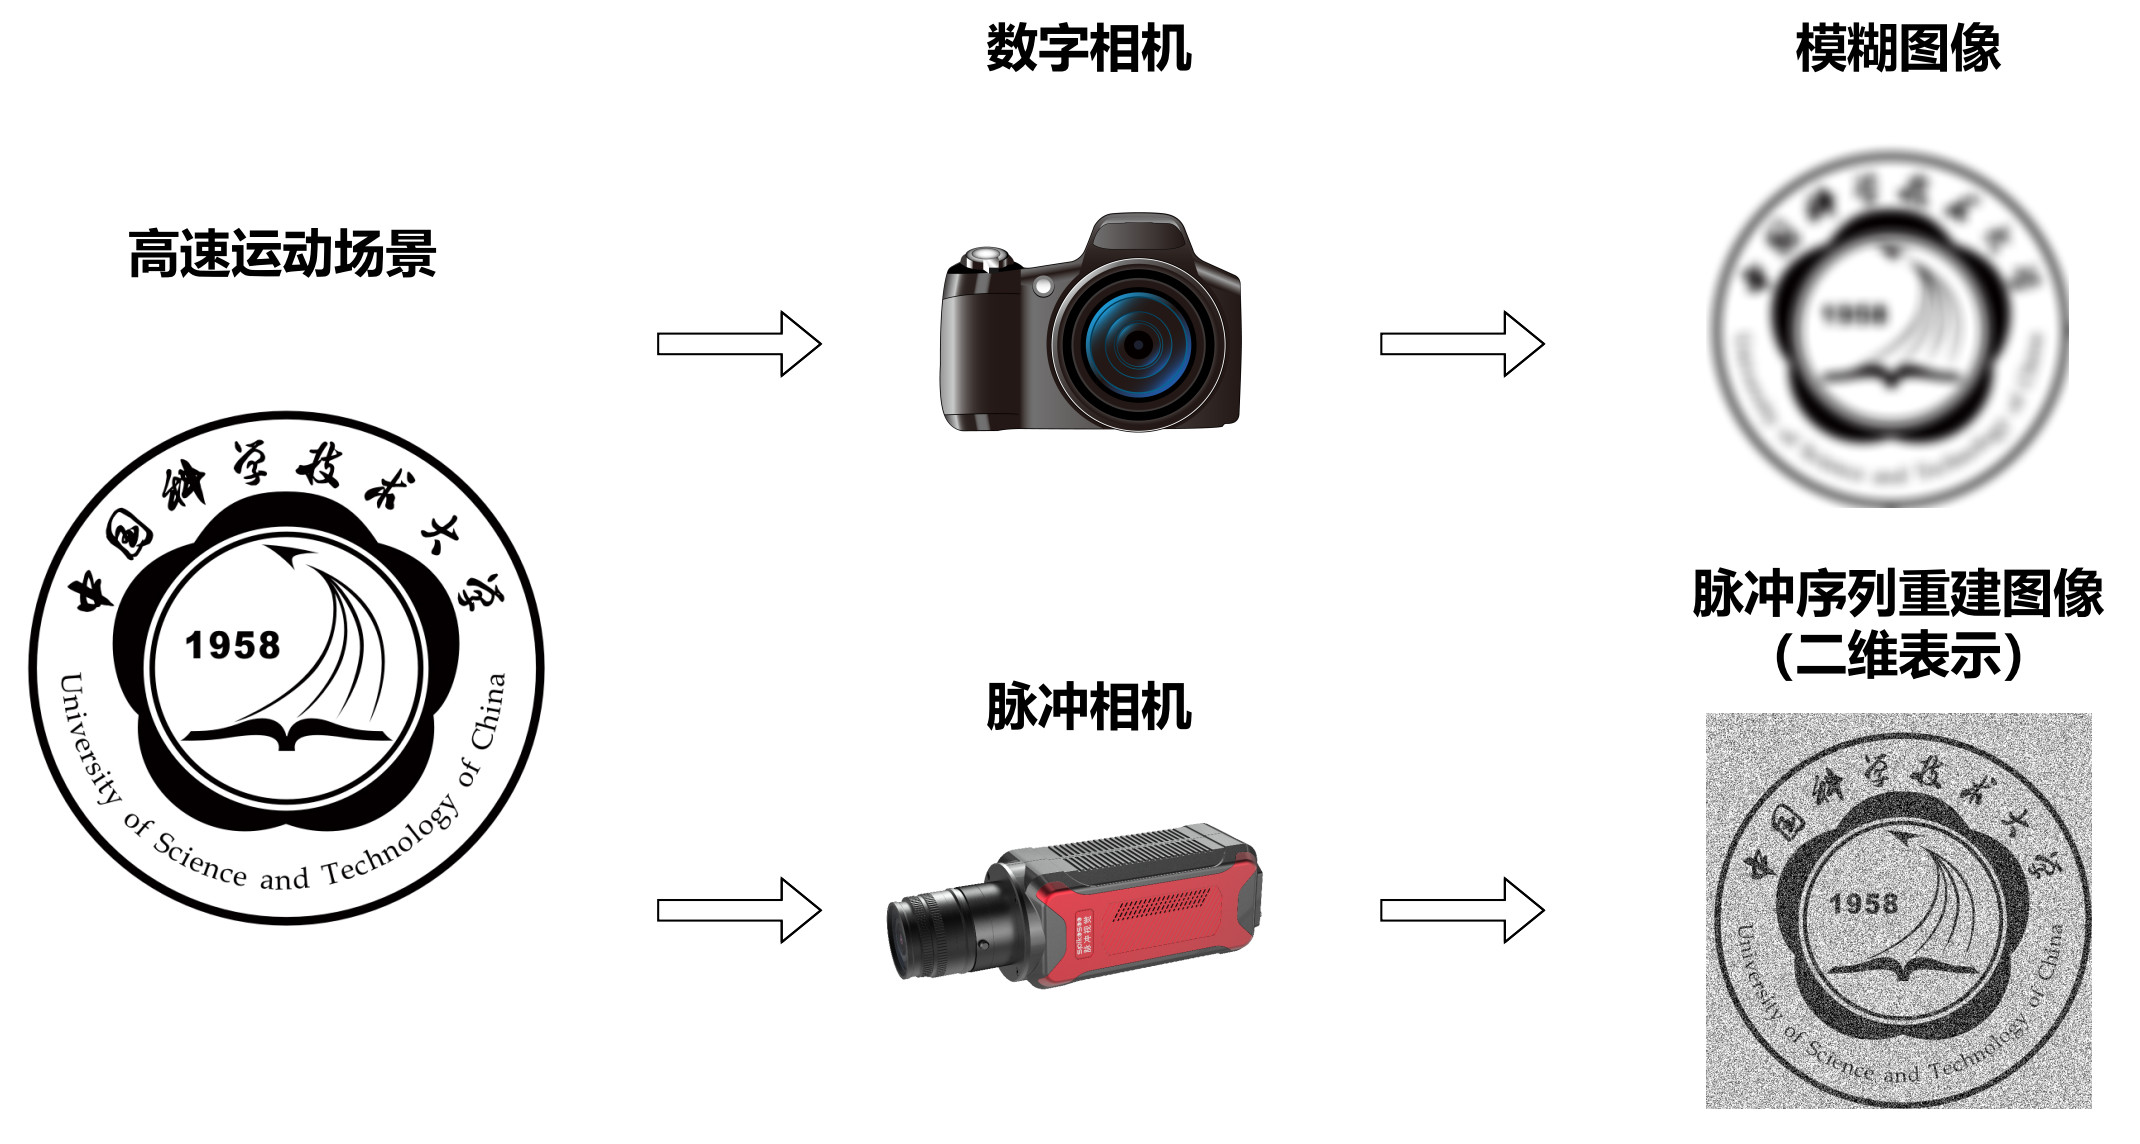
\includegraphics[width=\textwidth]{two_camera_result.jpg}
  \bicaption{图号、图题置于图的下方}{The English caption}
  \label{fig:two_camera_result}
\end{figure}    
%这里是插入一张图片的示意
\subsection{研究意义}



\section{研究问题定义}

\section{研究内容和成果}

\section{组织结构}



\section{脚注}

Lorem ipsum dolor sit amet, consectetur adipiscing elit, sed do eiusmod tempor
incididunt ut labore et dolore magna aliqua.
\footnote{Ut enim ad minim veniam, quis nostrud exercitation ullamco laboris
  nisi ut aliquip ex ea commodo consequat.
  Duis aute irure dolor in reprehenderit in voluptate velit esse cillum dolore
  eu fugiat nulla pariatur.}
